%%%%%%%%%%%%%%%%%%%%%%%%%%%%%%%%%%%%%%%%%
% Short Sectioned Assignment LaTeX Template Version 1.0 (5/5/12)
% This template has been downloaded from: http://www.LaTeXTemplates.com
% Original author:  Frits Wenneker (http://www.howtotex.com)
% License: CC BY-NC-SA 3.0 (http://creativecommons.org/licenses/by-nc-sa/3.0/)
%%%%%%%%%%%%%%%%%%%%%%%%%%%%%%%%%%%%%%%%%

%----------------------------------------------------------------------------------------
%	PACKAGES AND OTHER DOCUMENT CONFIGURATIONS
%----------------------------------------------------------------------------------------

\documentclass[paper=a4, fontsize=11pt]{scrartcl} % A4 paper and 11pt font size

% ---- Entrada y salida de texto -----

\usepackage[T1]{fontenc} % Use 8-bit encoding that has 256 glyphs
\usepackage[utf8]{inputenc}
%\usepackage{fourier} % Use the Adobe Utopia font for the document - comment this line to return to the LaTeX default

\usepackage{xcolor}
\usepackage{fancyhdr}
\usepackage{listings, lstautogobble}
\usepackage{comment}

\usepackage{subfigure} % subfiguras

%----------
\lstdefinestyle{customc}{
	belowcaptionskip=1\baselineskip,
	autogobble=true,
	breaklines=true,
	frame=L,
	xleftmargin=\parindent,
	language=C,
	showstringspaces=false,
	basicstyle=\footnotesize\ttfamily,
	keywordstyle=\bfseries\color{green!40!black},
	commentstyle=\itshape\color{purple!40!black},
	mathescape,
	identifierstyle=\color{blue},
	stringstyle=\color{orange},
}

\lstdefinestyle{bashmc}{
	frame=l,
	tabsize=2,
	breaklines=true,
	xleftmargin=\parindent,
	basicstyle=\ttfamily,
	showstringspaces=false,
	commentstyle=\color{red},
	keywordstyle=\color{blue},
	autogobble=true,
}

\lstdefinestyle{r}{
	belowcaptionskip=1\baselineskip,
	autogobble=true,
	breaklines=true,
	frame=L,
	xleftmargin=\parindent,
	language=C,
	showstringspaces=false,
	basicstyle=\footnotesize\ttfamily,
	keywordstyle=\bfseries\color{green!40!black},
	commentstyle=\itshape\color{purple!40!black},
	identifierstyle=\color{blue},
	mathescape,
	stringstyle=\color{orange},
}

\lstdefinestyle{r1}{
	frame=l,
	tabsize=2,
	breaklines=true,
	xleftmargin=\parindent,
	basicstyle=\ttfamily,
	showstringspaces=false,
	commentstyle=\color{red},
	keywordstyle=\color{blue},
	autogobble=true,
}




% ---- Idioma --------

\usepackage[spanish, es-tabla]{babel} % Selecciona el español para palabras introducidas automáticamente, p.ej. "septiembre" en la fecha y especifica que se use la palabra Tabla en vez de Cuadro

% ---- Otros paquetes ----
\usepackage{eurosym} % para el euro
\usepackage{url} % ,href} %para incluir URLs e hipervínculos dentro del texto (aunque hay que instalar href)
\usepackage{amsmath,amsfonts,amsthm} % Math packages
\usepackage{centernot}
%\usepackage{graphics,graphicx, floatrow} %para incluir imágenes y notas en las imágenes
\usepackage{graphics,graphicx, float} %para incluir imágenes y colocarlas

% Para hacer tablas comlejas
%\usepackage{multirow}
%\usepackage{threeparttable}

%\usepackage{sectsty} % Allows customizing section commands
%\allsectionsfont{\centering \normalfont\scshape} % Make all sections centered, the default font and small caps

\usepackage{fancyhdr} % Custom headers and footers
\pagestyle{fancyplain} % Makes all pages in the document conform to the custom headers and footers
\fancyhead{} % No page header - if you want one, create it in the same way as the footers below
\fancyfoot[L]{} % Empty left footer
\fancyfoot[C]{} % Empty center footer
\fancyfoot[R]{\thepage} % Page numbering for right footer
\renewcommand{\headrulewidth}{0pt} % Remove header underlines
\renewcommand{\footrulewidth}{0pt} % Remove footer underlines
\setlength{\headheight}{13.6pt} % Customize the height of the header

\numberwithin{equation}{section} % Number equations within sections (i.e. 1.1, 1.2, 2.1, 2.2 instead of 1, 2, 3, 4)
\numberwithin{figure}{section} % Number figures within sections (i.e. 1.1, 1.2, 2.1, 2.2 instead of 1, 2, 3, 4)
\numberwithin{table}{section} % Number tables within sections (i.e. 1.1, 1.2, 2.1, 2.2 instead of 1, 2, 3, 4)

\setlength\parindent{0pt} % Removes all indentation from paragraphs - comment this line for an assignment with lots of text

\newcommand{\horrule}[1]{\rule{\linewidth}{#1}} % Create horizontal rule command with 1 argument of height





%----------------------------------------------------------------------------------------
%	TÍTULO Y DATOS DEL ALUMNO
%----------------------------------------------------------------------------------------

\title{	
\normalfont \normalsize 
\textsc{\textbf{Metaheurísticas (2016-2017)} \\ Grado en Ingeniería Informática \\ Universidad de Granada} \\ [25pt] % Your university, school and/or department name(s)
\horrule{0.5pt} \\[0.4cm] % Thin top horizontal rule
\huge Practica 1: APC \\ % The assignment title
\horrule{2pt} \\[0.5cm] % Thick bottom horizontal rule
}

\author{Samuel Cardenete Rodríguez.  \\Correo: samuelcr1995@correo.ugr.es \\ DNI: 75934968P} % Nombre y apellidos

\date{\normalsize\today} % Incluye la fecha actual

%----------------------------------------------------------------------------------------
% DOCUMENTO
%----------------------------------------------------------------------------------------

\begin{document}

\maketitle % Muestra el Título

\newpage %inserta un salto de página

\tableofcontents % para generar el índice de contenidos

\listoffigures



\newpage





\section{Formulación del problema. APC}

\subsection{Introducción}
El problema a abordar en esta práctica consiste en el aprendizaje de pesos por características (APC). \\ 
Se trata de un problema de búsqueda con codificación real en el espacio n-dimensional, siendo n el número de características.\\ 

Estamos delante de un problema de Machine Learning, mediante el cuál dado un conjunto de datos no etiquetados obtengamos una etiqueta para cada uno de los datos (por ejemplo, determinar a partir de determinados parámetros si se tiene o no cáncer) bajo una tasa de acierto, siempre a maximizar.\\ 

\subsection{Objetivos}
Como objetivo principal del problema, ajustaremos un conjunto de ponderaciones o pesos asociados al conjunto total de características, utilizando para ello un conjunto de datos de entrenamiento (ya etiquetados), de tal forma que los clasificadores que se construyan a partir de él sean mejores.\\ 

APC asigna valores reales a las características, de tal forma que se describe o pondera la relevancia de cada una de ellas al problema del aprendizaje.

Para la resolución del problema, nos basaremos en optimizar el rendimiento de un clasificador basado en vecinos cercanos a partir de la inclusión de pesos asociados a las características del problema que modifican su valor en el momento de calcular las distancias entre ejemplos. En nuestro caso, el clasificador considerado será el 1-NN (vecino más cercano). Para ello adaptaremos las dos siguientes técnicas metaheurísticas:

\begin{itemize}
	\item Algoritmos Genéticos: Dos variantes generacionales elitistas (AGGs) y otras dos estacionarias (AGEs). Aparte del esquema de evolución, la única diferencia entre los dos modelos de AGGs y AGE será el operador de cruce empleado.
	
	\item Algoritmos Meméticos: Tres variantes de algoritmos meméticos (AMs) basadas en un AGG. La única diferencia entre las tres variantes de AMs serán los parámetros considerados para definir la aplicación de la búsqueda local.
\end{itemize}


Tras esto realizaremos un estudio comparativo de los resultados obtenidos por las distintas técnicas metaheurísticas.


\section{Algoritmos empleados al problema.}

\subsection{Algoritmos comunes}
Representación y explicación de los principales algoritmos comunes (operadores cruce, torneo binario...) así como su estructura en pseudocódigo.

\subsection{Generados soluciones aleatorias}
En el ámbito de nuestro problema APC, la representación de una solución corresponde a un vector de pesos W.
Para determinados algoritmos como los genéticos o la búsqueda local partimos de una solución aleatoria, es decir, un vector de pesos con componentes aleatorias generadas entre un intervalo $[0,1]$ (de esta forma ahorramos la normalización). El pseudocódigo sería el siguiente:

\begin{lstlisting}[ style=r]

Desde i hasta numero atributos
	SolucionInicialGenerarAleatorio $\Leftarrow$ Aleatorio (0,1)
Fin Desde

Devuelve SolucionInicial
\end{lstlisting}

De esta forma obtenemos un cromosoma aleatorio ya normalizado.

\subsection{Normalización de datos.}
Dados unos conjuntos de datos a utilizar como base de pruebas para nuestro problema (wdbc, sonar...), para no priorizar unos datos sobre otros es necesario la normalización de los datos en un intervalo $[0,1]$. Para ello, empleo un script en R, de forma que leemos los ficheros .arff, y utilizamos la función normalizarDatos para guardarlos en un .csv ya normalizados, de forma que dado un valor $x_j$ perteneciente a un atributo j del ejemplo $x$, y sabiendo que el dominio del atributo j es $[Min_j, Max_j]$, el valor normalizado de $x_j$ es:
\[
x_j^N = \frac{x_j -Min_j}{Max_j - Min_j}
\]

\subsection{Calcular distancia}
El clasificador empleado cuyo rendimiento pretendemos optimizar emplea la distancia euclídea entre dos características para el cálculo del vecino más cercano.\\ 
El pseudocódigo de la función que calcula la distancia entre dos características sería el siguiente:
\begin{lstlisting}[ style=r]
	//Calcular la distancia entre dos cromosomas
	// teniendo en cuenta el vector de pesos:
	Calcular distancia cromosoma A y B:
		Para cada i $\in$ Atributos(A) y j $\in$ Atributos(B)
			distancia = distancia + $\sqrt{Pesos_i*(i-j)^2}$
		Fin para cada
		
		Devolver distancia
\end{lstlisting}

De esta forma podemos utilizar dicha distancia para compararlas entre atributos y ver cual se encuentra más cerca del atributo actual.

\subsection{Función de evaluación}
Implementación de la función de evaluación 1-NN explicada en la descripción anteriormente.\\ 
El pseudocódigo es el siguiente:

\begin{lstlisting}[ style=r]
1-NN(train, test, pesos)

//Recorremos el conjunto test:
Para todo $a_i \in$ Test
	//inicializamos las distancias minimas al enemigo
	// y al amigo a infinito
	$d_{min} = \infty$

	
	//Ahora recorremos el conjunto train
	// calculando las distancias, buscando el min
	
	Para todo $b_i \in$ Train
		Si $a_i \neq b_i$ //leave one out
			Si (calculaDistancia($a_i$, $b_i$) < $d^{enemigo}_{min}$)
				$d_{min} =$ calculaDistancia($a_i$, $b_i$, pesos)
			
			Fin Si
	Fin para todo
	
	//Ahora calculamos la tasa:
	
	

Fin para todo

tasa = 100*etiquetas bien clasificadas / numero total de etiquetas

Devolver tasa
\end{lstlisting}


\subsection{Generación de vecinos}
En el esquema de generación de vecinos, necesario tanto para las mutaciones en los algoritmos genéticos, como para la generacion de vecindario en la búsqueda local, emplea un movimiento de cambio por mutación Normal, Mov(W,$\sigma$), deforma que a una característica del atributo se le suma un valor aleatorio obtenido apartir de una distribución normal de media 0 y desviación típica 0.3.\\ 

El pseudocódigo del algoritmo quedaría tal que así:

\begin{lstlisting}[ style=r]
Generar vecino (Pesos, $a_i$ = atributo a modificar)
	//Obtenemos un valor de la distribucion normal mencionada:
	aleatorio = Distribucion normal($media = 0$, $\sigma = 0.3$)
	//modificamos el atributo $a_i$ de los pesos:
	Pesos($a_i$) = Pesos($a_i$) + aleatorio
	
	//truncamos si es necesario para tener los valores normalizados 
	//entre $[0,1]$:
	
	Si Pesos($a_i$) < 0
		Pesos($a_i$) = 0
	Si Pesos($a_i$) > 1
		Pesos($a_i$) = 1
		
	Devolvemos Pesos
\end{lstlisting}
De esta forma tendremos un vecino generado.

\subsection{Operador cruce BLX}
Para el algoritmo genético BLX es necesario la implementación de dicho cruce BLX-$\alpha$, donde en nuestro caso $\alpha = 0.3$.
Dados dos cromosomas $p_1,  p_2$ pertenecientes a los padres, generamos dos descendientes $h_1, h_2$
de la siguiente forma descrita en pseudocódigo:

\begin{lstlisting}[ style=r]
CruceBLX entre $p_1$ y $p_2$
	//Obtenemos los atributos maximos y minimos para cada padre:
	$a_{max}^1 , a_{min}^1 \in p_1$
	$a_{max}^2, a_{min}^2 \in p_2$
	
	//Ahora obtenemos el maximo y el minimo de los dos padres:
	Max($a_{max}^1, a_{max}^2$)
	Min($a_{min}^1, a_{min}^2$)
	
	//Ahora generamos el intervalo I del cual generaremos aleatoriamente a los dos hijos:
	I = [Min($a_{min}^1, a_{min}^2$)-(Max($a_{max}^1, a_{max}^2$-Min($a_{min}^1, a_{min}^2$)*0.3,Max($a_{max}^1, a_{max}^2$)+(Max($a_{max}^1, a_{max}^2$-Min($a_{min}^1, a_{min}^2$)*0.3 ]
	
	//Creamos a los dos hijos $h_1,  h_2$
	Para cada atributo $a_1^i \in h_1$ y $a_2^i \in h_2$
		$a_1^i$ = Aleatorio (I)
		$a_2^i$ = Aleatorio (I)
	fin para cada
	
	devolvemos $a_1$ y $a_2$
		
\end{lstlisting}

De esta forma para cada pareja de padres, obtenemos una pareja de hijos.


\subsection{Operador cruce aritmético}
Además del operador BLX, es necesario implementar el operador de cruce aritmético. A diferencia del anterior, para cada pareja de padres obtenemos un único descendiente ($h_1$), que posee la media aritmética de los genes de ambos padres ($p_1$ y $p_2$).

\begin{lstlisting}[ style=r]
CruceAritmetico entre $p_1$ y $p_2$

	Para cada atributo $a_i \in h_1$
		$a_i$ = MediaAritmetica($a_{p1}^i$ y $a_{p2}^i$)
	fin para cada
	
	devolvemos $h_1$

\end{lstlisting}


\subsection{Torneo Binario}
La función torneo binario realiza un torneo entre dos padres (cromosomas) aleatorios, es decir, de entre esos dos padres, elige aquel que posea una mayor tasa de clasificación, o lo que es lo mismo, el mejor de los dos.\\ 
Genera tantos padres por torneo binario como se le indique. El pseudocódigo sería el siguiente, recibiendo una poblacion y sus tasas correspondientes:

\begin{lstlisting}[ style=r]

TorneoBinario Poblacion, Tasas
	Desde i hasta $N_{padres a generar}$
		//Obtenemos dos padres de forma aleatoria:
		p1 = aleatorio(Poblacion)
		p2 = aleatorio(Poblacion) distinto de p1
		
		//Ahora nos quedamos con el que tenga mejor tasa de los dos:
		mejores padres $\Leftarrow$ Max(Tasas(p1), Tasas(p2))
	Fin desde
	
	Devolver mejores padres

\end{lstlisting}

De esta forma obtenemos al final un número de padres deseados obtenidos mediante torneo binario, que emplearemos para un posterior cruce en los algoritmos genéticos y meméticos correspondientes.


\section{Estructuras de los principales métodos de búsqueda}

\subsection{Búsqueda Local}
La implementación de la búsqueda local consiste en emplear una técnica de búsqueda mediante explotación aplicada a nuestro problema, de forma que nos permita explotar una solución localmente, permitiendo así maximizar la tasa evaluación de una solución de forma local.\\ 

Como \textbf{criterio de parada} cuando se ejecute como algoritmo individual, se detendrá tras haber generado 20* (numero veces el número de características) vecinos, o cuando se hayan realizado 15000 evaluaciones (llamadas al 1-NN)

El pseudocódigo sería el siguiente:

\begin{lstlisting}[ style=r]

Busqueda Local (Conjunto de datos: Data)
	//Primero generamos una solucion inicial de forma aleatoria
	$S_{inicial} = GenerarSolucionAleatoria()$
	//Y calculamos la tasa
	$T_{inicial} =$ knn(Data, Data, $S_{inicial}$)
	
	
	//Inicializamos la primera como mejor solucion actual:
	$S_{mejor} = S_{inicial}$
	//Y guardamos la mejor tasa como esta:
	$T_{mejor} = T_{inicial}$
	
	//Llevamos cuenta del numero de evaluaciones que llevamos:
	numero evaluaciones = 1
	
	
	//Empezamos a generar vecindario con la solucion actual 
	// hasta que se cumplan los criterios de parada:

	Mientras (numero evaluaciones < 15000) y (vecinos generados < 20*(Numero genes cromosoma)
	
		//vamos generando el vecindario:
		Si hay_que_generar_nuevo_vecindario
			//rellenamos una cola de indices aleatorios desde con los genes a mutar
			vecinos por generar = Shuffle(Indices de genes)
			hay_que_generar_nuevo_vecindario = false
		Sino
			//Generamos un vecino correspondiente sacando
			// un elemento de la cola anterior para
			//Indicar que gen mutar:
			nuevo vecino = generarVecino($S_{mejor}$, vecinos por generar)
			vecinos generados +1
			
			Si (Tasa(nuevo vecino) > $T_{mejor}$)
				$S_{mejor}$ = nuevo vecino
				$T_{mejor}$ = knn(Data, Data, nuevo vecino)
				
				numero evaluaciones+1
				
				//Indicamos que genere un nuevo vecindario
				hay_que_generar_nuevo_vecindario = true
			Fin Si
			
		Fin Sino
		
		//Hemos recorrido un vecindario sin mejora
		Si estaVacia(vecinos por generar)
			hay_que_generar_nuevo_vecindario = true
		Fin Si
		
	Fin Mientras
	
	Devolver $S_{mejor}$
\end{lstlisting}


\subsection{Algortimos genéticos}

\subsubsection{AGG BLX}
El AGG BLX se trata de un algoritmo que implementa un esquema de evolución generacional elitista, mediante un esquema de reemplazamiento generacional, es decir, la nueva generación reemplaza en cada iteración completamente a la generación actual.\\ 
Como operador de selección se implementará el torneo binario ya descrito anteriormente, para la elección de los mejores padres a cruzar.\\ 

El operador de cruce es el BLX, descrito anteriormente, para generar en cada cruce a partir de dos padres dos descendientes. La probabilidad de cruce será de 0.7.\\ 

Para la mutación, se empleará la función generarVecino descrita anteriormente, bajo una probabilidad de mutación en población de un 0.001.\\ 

Por último el criterio de parada del algoritmo es no superar las 15000 evaluaciones de la función objetivo (1-NN).

\begin{lstlisting}[ style=r]

AGG BLX (Data)
	//Creamos una poblacion de 30 individuos aleatoria:
	Desde i = 0 hasta i < 30
		Poblacion actual <- generaSolucionAleatoria()
	Fin Desde
	
	Para cada $P_i \in $ poblacion actual
		tasas actuales $\Leftarrow$ knn(Data, $P_i$)
	Fin para cada
	
	//empezamos generacion tras generacion hasta cumplir
	//El criterio de parada:
	Mientras (num. evaluaciones < 15000)
		//Calculamos el mejor padre de la poblacion actual:
		$Padre_{mejor}$ = Max(tasas poblacion actual)
		
		//Obtenemos los padres (parejas) a cruzar, 
		//con una probabilidad de cruce del 70%
		parejas a cruzar = 0.7 * 30/2
		
		//Llamamos al torneo binario, obteniendo los padres deseados
		padres a cruzar = torneoBinario(poblacion actual)
		//Realizamos los cruces, obteniendo dos hijos por cruce
		Desde i = 0 hasta i < parejas a cruzar
			nueva poblacion $\Leftarrow$ cruceBLX($pareja_i, pareja_{i+1}$)
		Fin Desde
		
		//Aniadimos los padres que no se han cruzado hasta llegar 
		// a una nueva poblacion de 30:
		Mientras Tam(nueva poblacion) < 30
			nueva poblacion $\Leftarrow$ padres no se han cruzado
		Fin Mientras
		
		//Calculamos el numero de individuos a mutar, con
		// una probabilidad de 0.001:
		individuos a mutar = 0.001 * 30
		
		//Mutamos de forma aleatoria los n individuos a mutar:
		Desde i = 0 hasta i < individuos a mutar
			nueva $poblacion_{aleatorio}$ = generarVecino (nueva $poblacion_{aleatorio}$)
		Fin Desde
		
		//Calculamos las tasas de la nueva poblacion
		Para cada $P_i \in $ nueva poblacion
			nuevas tasas $\Leftarrow$ knn(Data, $P_i$)
		Fin para cada
		
		//Si hemos perdido al mejor padre lo cambiamos por 
		//el peor de la poblacion.
		Si (hemos perdido al mejor padre)
			Min(tasas actual) = mejor padre
		Fin Si
		
		//La nueva poblacion es ahora la actual:
		poblacion actual = nueva poblacion
		tasas actual = nuevas tasas
	
	
	Fin Mientras
	
	Devolver mejor individuo poblacion actual
\end{lstlisting}


\subsubsection{AGG CA}
El AGG CA se trata de un algoritmo que implementa un esquema de evolución generacional elitista, mediante un esquema de reemplazamiento generacional, es decir, la nueva generación reemplaza en cada iteración completamente a la generación actual.\\ 
Como operador de selección se implementará el torneo binario ya descrito anteriormente, para la elección de los mejores padres a cruzar.\\ 

El operador de cruce es el CA, descrito anteriormente, para generar en cada cruce a partir de dos padres un descendiente. La probabilidad de cruce será de 0.7.\\ 

Para la mutación, se empleará la función generarVecino descrita anteriormente, bajo una probabilidad de mutación en población de un 0.001.\\ 

Por último el criterio de parada del algoritmo es no superar las 15000 evaluaciones de la función objetivo (1-NN).


\begin{lstlisting}[ style=r]

AGG CA (Data)
	//Creamos una poblacion de 30 individuos aleatoria:
	Desde i = 0 hasta i < 30
		Poblacion actual <- generaSolucionAleatoria()
	Fin Desde
	
	Para cada $P_i \in $ poblacion actual
		tasas actuales $\Leftarrow$ knn(Data, Data, $P_i$)
	Fin para cada
	
	//empezamos generacion tras generacion hasta cumplir
	//El criterio de parada:
	Mientras (num. evaluaciones < 15000)
		//Calculamos el mejor padre de la poblacion actual:
		$Padre_{mejor}$ = Max(tasas poblacion actual)
		
		//Obtenemos los padres (parejas) a cruzar, 
		//con una probabilidad de cruce del 70%
		parejas a cruzar = 0.7 * 30
		
		//Llamamos al torneo binario, obteniendo los padres deseados, 
		// en este caso, el doble del tamanio de la poblacion actual, puesto que 
		// el operador de cruce CA devuelve un unico descendiente.
		padres a cruzar = torneoBinario(poblacion actual)
		//Realizamos los cruces, obteniendo dos hijos por cruce
		Desde i = 0 hasta i < parejas a cruzar
			nueva poblacion $\Leftarrow$ cruceAritmetico($pareja_i, pareja_{i+1}$)
		Fin Desde
		
		//Aniadimos los padres que no se han cruzado hasta llegar 
		// a una nueva poblacion de 30:
		Mientras Tam(nueva poblacion) < 30
			nueva poblacion $\Leftarrow$ padres no se han cruzado
		Fin Mientras
		
		//Calculamos el numero de individuos a mutar, con
		// una probabilidad de 0.001:
		individuos a mutar = 0.001 * 30
		
		//Mutamos de forma aleatoria los n individuos a mutar:
		Desde i = 0 hasta i < individuos a mutar
			nueva $poblacion_{aleatorio}$ = generarVecino (nueva $poblacion_{aleatorio}$)
		Fin Desde
		
		//Calculamos las tasas de la nueva poblacion
		Para cada $P_i \in $ nueva poblacion
			nuevas tasas $\Leftarrow$ knn(Data, Data, $P_i$)
		Fin para cada
		
		//Si hemos perdido al mejor padre lo cambiamos por 
		//el peor de la poblacion.
		Si (hemos perdido al mejor padre)
			Min(tasas actual) = mejor padre
		Fin Si
		
		//La nueva poblacion es ahora la actual:
		poblacion actual = nueva poblacion
		tasas actual = nuevas tasas
		
	
	Fin Mientras
	
	Devolver mejor individuo poblacion actual
\end{lstlisting}


\subsubsection{AGE BLX}
El AGE BLX se trata de un algoritmo que implementa un esquema de evolución estacionario, mediante un esquema de reemplazamiento en el que los dos hijos de la nueva generación compite con los dos peores individuos de la generación actual, reemplazando a estos en caso de ser mejores.\\ +

Como operador de selección se implementará el torneo binario ya descrito anteriormente, para la elección de los mejores padres a cruzar.\\ 

El operador de cruce es el BLX, descrito anteriormente, para generar en cada cruce a partir de dos padres dos descendientes. La probabilidad de cruce será de 0.7.\\ 

Para la mutación, se empleará la función generarVecino descrita anteriormente, bajo una probabilidad de mutación en población de un 0.001.\\ 

Por último el criterio de parada del algoritmo es no superar las 15000 evaluaciones de la función objetivo (1-NN).

\begin{lstlisting}[ style=r]
AGE BLX (Data)
	//Creamos una poblacion de 30 individuos aleatoria:
	Desde i = 0 hasta i < 30
		Poblacion actual <- generaSolucionAleatoria()
	Fin Desde
	
	Para cada $P_i \in $ poblacion actual
		tasas actuales $\Leftarrow$ knn(Data, $P_i$)
	Fin para cada
	
	//empezamos generacion tras generacion hasta cumplir
	//El criterio de parada:
	Mientras (num. evaluaciones < 15000)
		//Calculamos el mejor padre de la poblacion actual:
		$Padre_{mejor}$ = Max(tasas poblacion actual)
		
		//Obtenemos los padres (parejas) a cruzar, 
		//con una probabilidad de cruce del 1, es decir
		// unicamente cruzamos 1 pareja:
		num parejas = 1
		
		//Llamamos al torneo binario, obteniendo los padres deseados
		padres a cruzar = torneoBinario(poblacion actual)
		//Realizamos los cruces, obteniendo dos hijos
		
		 $h_1, h_2$ $\Leftarrow$ cruceBLX($pareja_0, pareja_{1}$)
	
		//Igualamos la nueva poblacion a la poblacion actual:
		nueva poblacion = poblacion actual
		nueva tasas = tasas actual
		//Calculamos el numero de individuos a mutar, con
		// una probabilidad de 0.001:
		individuos a mutar = 0.001 * 30
		
		//Mutamos de forma aleatoria los n individuos a mutar:
		Desde i = 0 hasta i < individuos a mutar
			nueva $poblacion_{aleatorio}$ = generarVecino (nueva $poblacion_{aleatorio}$)
		Fin Desde
		
		//Comparamos los dos hijos $h_1$ y $h_2$ con los dos peores de la poblacion:
		Si (Tasa($h_1$) > peoresDosIndividuos(poblacion actual))
			//sustituimos los individuos:
			nueva poblacion(peor individuo1) = h_1
			// y sus tasas
			Tasa(peor individuo1) = Tasa($h_1$)
		Fin Si
		
		Si (Tasa($h_2$) > peoresDosIndividuos(poblacion actual))
			//sustituimos los individuos:
			nueva poblacion(peor individuo2) = h_2
			// y sus tasas
			Tasa(peor individuo2) = Tasa($h_2$)
		Fin Si
		
		//La nueva poblacion es ahora la actual:
		poblacion actual = nueva poblacion
		tasas actual = nuevas tasas
		
	
	Fin Mientras
	
	Devolver mejor individuo poblacion actual
\end{lstlisting}



\subsubsection{AGE CA}
El AGE CA se trata de un algoritmo que implementa un esquema de evolución estacionario, mediante un esquema de reemplazamiento en el que los dos hijos de la nueva generación compite con los dos peores individuos de la generación actual, reemplazando a estos en caso de ser mejores.\\ +

Como operador de selección se implementará el torneo binario ya descrito anteriormente, para la elección de los mejores padres a cruzar.\\ 

El operador de cruce es el CA, descrito anteriormente, para generar en cada cruce a partir de dos padres dos descendientes. La probabilidad de cruce será de 0.7.\\ 

Para la mutación, se empleará la función generarVecino descrita anteriormente, bajo una probabilidad de mutación en población de un 0.001.\\ 

Por último el criterio de parada del algoritmo es no superar las 15000 evaluaciones de la función objetivo (1-NN).


\begin{lstlisting}[ style=r]
AGE CA (Data)
	//Creamos una poblacion de 30 individuos aleatoria:
	Desde i = 0 hasta i < 30
		Poblacion actual <- generaSolucionAleatoria()
	Fin Desde
	
	Para cada $P_i \in $ poblacion actual
		tasas actuales $\Leftarrow$ knn(Data, $P_i$)
	Fin para cada
	
	//empezamos generacion tras generacion hasta cumplir
	//El criterio de parada:
	Mientras (num. evaluaciones < 15000)
		//Calculamos el mejor padre de la poblacion actual:
		$Padre_{mejor}$ = Max(tasas poblacion actual)
		
		//Obtenemos los padres (parejas) a cruzar, 
		//con una probabilidad de cruce del 1, es decir
		// unicamente cruzamos 2 parejas para obtener 2 hijos:
		num parejas = 2
		
		//Llamamos al torneo binario, obteniendo los padres deseados
		padres a cruzar = torneoBinario(poblacion actual)
		//Realizamos los cruces, obteniendo dos hijos
		
		$h_1$ $\Leftarrow$ cruceCA($pareja_0, pareja_{1}$)
		$h_2$ $\Leftarrow$ cruceCA($pareja_2, pareja_{3}$)
		
		//Igualamos la nueva poblacion a la poblacion actual:
		nueva poblacion = poblacion actual
		nueva tasas = tasas actual
		//Calculamos el numero de individuos a mutar, con
		// una probabilidad de 0.001:
		individuos a mutar = 0.001 * 30
		
		//Mutamos de forma aleatoria los n individuos a mutar:
		Desde i = 0 hasta i < individuos a mutar
			nueva $poblacion_{aleatorio}$ = generarVecino (nueva $poblacion_{aleatorio}$)
		Fin Desde
		
		//Comparamos los dos hijos $h_1$ y $h_2$ con los dos peores de la poblacion:
		Si (Tasa($h_1$) > peoresDosIndividuos(poblacion actual))
			//sustituimos los individuos:
			nueva poblacion(peor individuo1) = h_1
			// y sus tasas
			Tasa(peor individuo1) = Tasa($h_1$)
		Fin Si
		
		Si (Tasa($h_2$) > peoresDosIndividuos(poblacion actual))
			//sustituimos los individuos:
			nueva poblacion(peor individuo2) = h_2
			// y sus tasas
			Tasa(peor individuo2) = Tasa($h_2$)
		Fin Si
		
		//La nueva poblacion es ahora la actual:
		poblacion actual = nueva poblacion
		tasas actual = nuevas tasas


	Fin Mientras
	
	Devolver mejor individuo poblacion actual
\end{lstlisting}



\subsection{Algoritmos meméticos}
La implementación realizada para los algoritmos meméticos consiste en hibridar los algoritmos generacionales anteriormente analizados que mejor resultado me han dado, en mi caso, el AGG-CA, incluyendo en este un proceso de búsqueda local para obtener, aparte de la exploración proporcionada por el algoritmo genético, tener también una explotación mediante el uso de dicha búsqueda local.\\ 

Utilizaremos para los meméticos una población de tamaño 10.

Estudiaremos las tres posibilidades de hibridación siguientes:

\subsubsection{AM-(10, 1.0)}
Consiste en que dado el algoritmo AGG-CA mencionado, cada 10 generaciones aplicamos una búsqueda local sobre todos los cromosomas de la población, mejorando cada cromosoma así de forma local.\\ 

El pseudocódigo sería el siguiente:



\begin{lstlisting}[ style=r]

AM-(10, 1.0) (Data)
//Creamos una poblacion de 10 individuos aleatoria:
Desde i = 0 hasta i < 10
	Poblacion actual <- generaSolucionAleatoria()
Fin Desde

Para cada $P_i \in $ poblacion actual
	tasas actuales $\Leftarrow$ knn(Data, Data, $P_i$)
Fin para cada

//empezamos generacion tras generacion hasta cumplir
//El criterio de parada:
Mientras (num. evaluaciones < 15000)
	//Calculamos el mejor padre de la poblacion actual:
	$Padre_{mejor}$ = Max(tasas poblacion actual)
	
	//Obtenemos los padres (parejas) a cruzar, 
	//con una probabilidad de cruce del 70%
	parejas a cruzar = 0.7 * 10
	
	//Llamamos al torneo binario, obteniendo los padres deseados, 
	// en este caso, el doble del tamanio de la poblacion actual, puesto que 
	// el operador de cruce CA devuelve un unico descendiente.
	padres a cruzar = torneoBinario(poblacion actual)
	//Realizamos los cruces, obteniendo dos hijos por cruce
	Desde i = 0 hasta i < parejas a cruzar
		nueva poblacion $\Leftarrow$ cruceAritmetico($pareja_i, pareja_{i+1}$)
	Fin Desde
	
	//Aniadimos los padres que no se han cruzado hasta llegar 
	// a una nueva poblacion de 10:
	Mientras Tam(nueva poblacion) < 10
		nueva poblacion $\Leftarrow$ padres no se han cruzado
	Fin Mientras
	
	//Calculamos el numero de individuos a mutar, con
	// una probabilidad de 0.001:
	individuos a mutar = 0.001 * 10
	
	//Mutamos de forma aleatoria los n individuos a mutar:
	Desde i = 0 hasta i < individuos a mutar
		nueva $poblacion_{aleatorio}$ = generarVecino (nueva $poblacion_{aleatorio}$)
	Fin Desde
	
	//Calculamos las tasas de la nueva poblacion
	Para cada $P_i \in $ nueva poblacion
		nuevas tasas $\Leftarrow$ knn(Data, Data, $P_i$)
	Fin para cada
	
	//Si hemos perdido al mejor padre lo cambiamos por 
	//el peor de la poblacion.
	Si (hemos perdido al mejor padre)
		Min(tasas actual) = mejor padre
	Fin Si
	
	//La nueva poblacion es ahora la actual:
	poblacion actual = nueva poblacion
	tasas actual = nuevas tasas
	
	
	//Si ya llevamos 10 generaciones aplicamos la busqueda local:
	Si (generaciones es multiplo de 10)
		Para cada $c_i$ \in poblacion actual
			$c_i$ = BL (Data, $c_1$)
			Tasas actual ($c_i$) = Tasa($c_i$)
		Fin para cada
	Fin Si
	

Fin Mientras


Devolver mejor individuo poblacion actual
\end{lstlisting}


\subsubsection{AM-(10, 0.1)}
Consiste en que dado el algoritmo AGG-CA mencionado, cada 10 generaciones aplicamos una búsqueda local sobre un 10\% aleatorio de los cromosomas de la población.\\ 
El pseudocódigo sería el siguiente:



\begin{lstlisting}[ style=r]

AM-(10, 0.1) (Data)
//Creamos una poblacion de 10 individuos aleatoria:
Desde i = 0 hasta i < 10
	Poblacion actual <- generaSolucionAleatoria()
Fin Desde

Para cada $P_i \in $ poblacion actual
	tasas actuales $\Leftarrow$ knn(Data, Data, $P_i$)
Fin para cada

//empezamos generacion tras generacion hasta cumplir
//El criterio de parada:
Mientras (num. evaluaciones < 15000)
	//Calculamos el mejor padre de la poblacion actual:
	$Padre_{mejor}$ = Max(tasas poblacion actual)
	
	//Obtenemos los padres (parejas) a cruzar, 
	//con una probabilidad de cruce del 70%
	parejas a cruzar = 0.7 * 10
	
	//Llamamos al torneo binario, obteniendo los padres deseados, 
	// en este caso, el doble del tamanio de la poblacion actual, puesto que 
	// el operador de cruce CA devuelve un unico descendiente.
	padres a cruzar = torneoBinario(poblacion actual)
	//Realizamos los cruces, obteniendo dos hijos por cruce
	Desde i = 0 hasta i < parejas a cruzar
		nueva poblacion $\Leftarrow$ cruceAritmetico($pareja_i, pareja_{i+1}$)
	Fin Desde
	
	//Aniadimos los padres que no se han cruzado hasta llegar 
	// a una nueva poblacion de 10:
	Mientras Tam(nueva poblacion) < 10
		nueva poblacion $\Leftarrow$ padres no se han cruzado
	Fin Mientras
	
	//Calculamos el numero de individuos a mutar, con
	// una probabilidad de 0.001:
	individuos a mutar = 0.001 * 10
	
	//Mutamos de forma aleatoria los n individuos a mutar:
	Desde i = 0 hasta i < individuos a mutar
		nueva $poblacion_{aleatorio}$ = generarVecino (nueva $poblacion_{aleatorio}$)
	Fin Desde
	
	//Calculamos las tasas de la nueva poblacion
	Para cada $P_i \in $ nueva poblacion
		nuevas tasas $\Leftarrow$ knn(Data, Data, $P_i$)
	Fin para cada
	
	//Si hemos perdido al mejor padre lo cambiamos por 
	//el peor de la poblacion.
	Si (hemos perdido al mejor padre)
		Min(tasas actual) = mejor padre
	Fin Si
	
	//La nueva poblacion es ahora la actual:
	poblacion actual = nueva poblacion
	tasas actual = nuevas tasas
	
	
	//Si ya llevamos 10 generaciones aplicamos la busqueda local:
	Si (generaciones es multiplo de 10)
		Para cada $c_i$ \in 0.1* mejores poblacion actual
			$c_i$ = BL (Data, $c_1$)
			Tasas actual ($c_i$) = Tasa($c_i$)
		Fin para cada
	Fin Si


Fin Mientras

Devolver mejor individuo poblacion actual
\end{lstlisting}



\subsubsection{AM-(10, 0.1mej)}
Consiste en que dado el algoritmo AGG-CA mencionado, cada 10 generaciones aplicamos una búsqueda local sobre los 0.1*N mejores cromosomas de la población.\\ 
El pseudocódigo sería el siguiente:


\begin{lstlisting}[ style=r]

AM-(10, 0.1mej) (Data)
//Creamos una poblacion de 10 individuos aleatoria:
Desde i = 0 hasta i < 10
	Poblacion actual <- generaSolucionAleatoria()
Fin Desde

Para cada $P_i \in $ poblacion actual
	tasas actuales $\Leftarrow$ knn(Data, Data, $P_i$)
Fin para cada

//empezamos generacion tras generacion hasta cumplir
//El criterio de parada:
Mientras (num. evaluaciones < 15000)
	//Calculamos el mejor padre de la poblacion actual:
	$Padre_{mejor}$ = Max(tasas poblacion actual)
	
	//Obtenemos los padres (parejas) a cruzar, 
	//con una probabilidad de cruce del 70%
	parejas a cruzar = 0.7 * 10
	
	//Llamamos al torneo binario, obteniendo los padres deseados, 
	// en este caso, el doble del tamanio de la poblacion actual, puesto que 
	// el operador de cruce CA devuelve un unico descendiente.
	padres a cruzar = torneoBinario(poblacion actual)
	//Realizamos los cruces, obteniendo dos hijos por cruce
	Desde i = 0 hasta i < parejas a cruzar
		nueva poblacion $\Leftarrow$ cruceAritmetico($pareja_i, pareja_{i+1}$)
	Fin Desde
	
	//Aniadimos los padres que no se han cruzado hasta llegar 
	// a una nueva poblacion de 10:
	Mientras Tam(nueva poblacion) < 10
		nueva poblacion $\Leftarrow$ padres no se han cruzado
	Fin Mientras
	
	//Calculamos el numero de individuos a mutar, con
	// una probabilidad de 0.001:
	individuos a mutar = 0.001 * 10
	
	//Mutamos de forma aleatoria los n individuos a mutar:
	Desde i = 0 hasta i < individuos a mutar
		nueva $poblacion_{aleatorio}$ = generarVecino (nueva $poblacion_{aleatorio}$)
	Fin Desde
	
	//Calculamos las tasas de la nueva poblacion
	Para cada $P_i \in $ nueva poblacion
		nuevas tasas $\Leftarrow$ knn(Data, Data, $P_i$)
	Fin para cada
	
	//Si hemos perdido al mejor padre lo cambiamos por 
	//el peor de la poblacion.
	Si (hemos perdido al mejor padre)
		Min(tasas actual) = mejor padre
	Fin Si
	
	//La nueva poblacion es ahora la actual:
	poblacion actual = nueva poblacion
	tasas actual = nuevas tasas
	
	
	//Si ya llevamos 10 generaciones aplicamos la busqueda local:
	Si (generaciones es multiplo de 10)
		Para cada $c_i$ \in 0.1*poblacion actual
			$c_i$ = BL (Data, $c_1$)
			Tasas actual ($c_i$) = Tasa($c_i$)
		Fin para cada
	Fin Si


Fin Mientras


Devolver mejor individuo poblacion actual
\end{lstlisting}



\section{Algoritmo de comparación}
En el dominio del problema a tratar, la implementación de un método de comparación se realiza mediante el método RELIEF.

Se trata de una solución de tipo Greedy.

Dicho método partimos de un vector de pesos inicializado a 0 inicialmente y en cada paso modificamos dichos pesos en función, para cada uno de los ejemplos del conjunto de entrenamiento, de su enemigo más cercano y su amigo más cercano.\\ 

Definimos el enemigo más cercano como aquel ejemplo con clase diferente que se encuentra a menor distancia euclídea; y el amigo más cercano de la misma forma pero que tiene la misma clase que él.
NUNCA COMPARAMOS LA DISTANCIA ENTRE EL CONSIGO MISMO (Leave one out), sino obtendríamos siempre una tasa cercana al 100\%

Tras el cálculo de W, y si es necesario, se normaliza W.

El pseudocódigo sería el siguiente:




\begin{lstlisting}[ style=r]
RELIEF(train, test)
	//Inicializamos los pesos a 0:
	Para todo $w_i \in$ w
		$w_i$ = 0
	Fin para todo
	
	//Recorremos el conjunto test:
	Para todo $a_i \in$ Test
		//inicializamos las distancias minimas al enemigo
		// y al amigo a infinito
		$d^{amigo}_{min} = \inf$
		$d^{enemigo}_{min} = \inf$
		
		//Ahora recorremos el conjunto train
		// calculando las distancias, buscando el min amigo
		// y enemigo:
		
		Para todo $b_i \in$ Train
			Si $a_i \neq b_i$ //leave one out
				Si etiqueta($b_i \neq a_i$) && (calculaDistancia($a_i$, $b_i$) < $d^{enemigo}_{min}$)
					$d^{enemigo}_{min} =$ calculaDistancia($a_i$, $b_i$)
					
				Sino Si(calculaDistancia($a_i$, $b_i$) < $d^{enemigo}_{min}$)
					$d^{amigo}_{min} =$ calculaDistancia($a_i$, $b_i$)
			Fin para todo
		Fin para todo
		
		//Ahora actualizamos los pesos
		w = w + $|a_i - a^{enemigo}| - |a_i - a_{amigo}|$
		
	Fin para todo
	
	
	Devolver W
\end{lstlisting}


\section{Procedimiento para la realización de la práctica}
Para la realización de la práctica no he hecho uso de ningúna implementación ni código externos, todo ha sido desarrollado por mi mismo.\\ 

\subsection{Manual de usuario}
Si se desea realizar una réplica de las pruebas aquí descritas serán necesarios los siguientes pasos:

\begin{enumerate}
	\item En primer lugar, será necesario ejecutar el script en R ''practica1.R'', cuya función es leer los archivos que se encuentran en formato '.arff', normalizarlos, y escribirlos en ficheros '.csv' (almacenados en la carpeta ''datos'') para facilitar de esta forma la futura lectura.
	
	\item Una vez tenemos los datos normalizados, ejecutar el makefile incluido, de esta forma obtendremos un ejecutable ''practica1''.
	
	\item Por último lanzar dicho programa, indicando como argumento el nombre del conjunto de datos que se desea utilizar para la realización de los algoritmos, por ejemplo: ''./practica1 cancer'', de esta forma utilizaríamos la base de datos de cáncer de mama.
	
	\item Tras esto se ejecutarán TODOS los algoritmos indicando tanto la tasa obtenida para cada uno, como los tiempos, la tasa media de todas las particiones y su correspondiente tiempo medio.
\end{enumerate}


\section{Experimentos y análisis de resultados}

Para la realización de los experimento utilizaremos 3 conjuntos de datos distintos, uno para predecir si se posee cáncer de mama, otro para detectar posible correo 'spam' y un tercero, para clasificar datos de un sonar.\\ 

Cómo método de validación utilizaremos el método 5x2-cross validation (cv). Para ello, se generarán 5 particiones distintas del conjunto de datos proporcionado en subconjuntos de entrenamiento y prueba realizadas al 50\%. Para cada partición, se aprenderá primero el clasificador con una parte y se validará con la otra y viceversa, resultando en 10 ejecuciones de cada algoritmo sobre cada conjunto de datos.\\ 

Cómo medida de validación, utilizaremos la tasa de acierto del clasificador 1-NN sobre el conjunto de prueba. El resultado final será la media de los 10 valores obtenidos, uno para cada ejecución del algoritmo.\\ 

También emplearemos cómo método de comparación el tiempo de ejecución empleado por cada uno.
Las semillas utilizadas para la realización de todas las pruebas son las siguientes:
\begin{verbatim}
	
	default_random_engine generator (5); //para los números aleatorios
	normal_distribution<double> distribution (0.0,0.3); //para la distribución normal
\end{verbatim} 
Los tiempos obtenidos y las tasas para cada algoritmo de forma individual son las siguientes:

\begin{figure}[H]
	\centering
	\caption{Resultados 1NN} \label{fig: Resultados 1NN}
	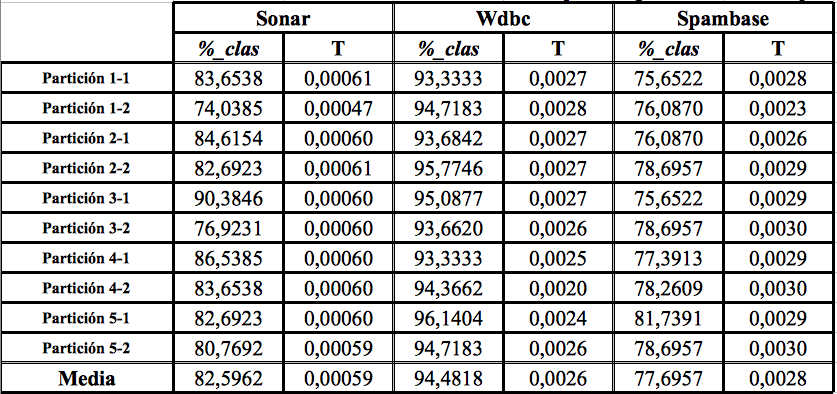
\includegraphics[scale=0.55]{1NN.png}  
	
\end{figure}

\begin{figure}[H]
	\centering
	\caption{Resultados RELIEF} \label{fig: Resultados RELIEF}
	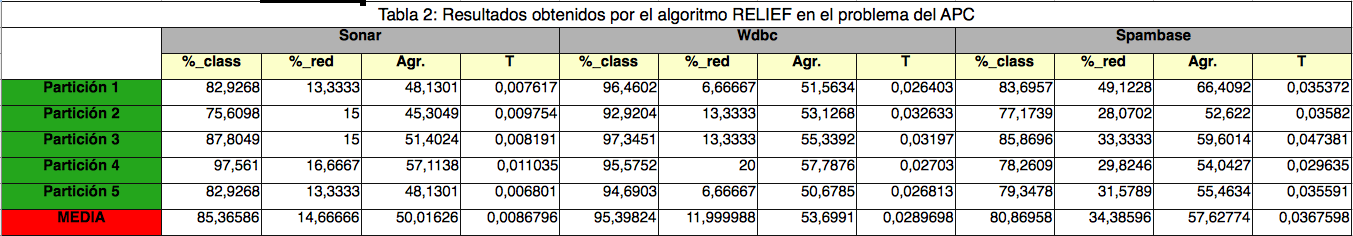
\includegraphics[scale=0.55]{RELIEF.png}  
	
\end{figure}

\begin{figure}[H]
	\centering
	\caption{Resultados BL} \label{fig: Resultados BL}
	\includegraphics[scale=0.55]{BL.png}  
	
\end{figure}

\begin{figure}[H]
	\centering
	\caption{Resultados AGG-BLX} \label{fig: Resultados AGG-BLX}
	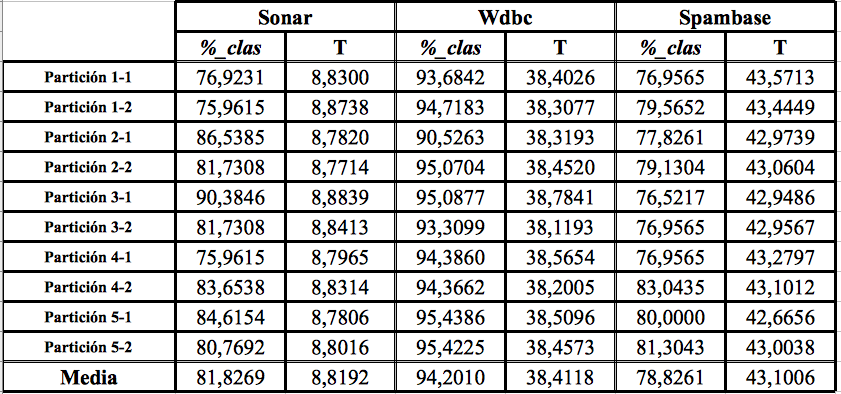
\includegraphics[scale=0.55]{AGG-BLX.png}  
	
\end{figure}

\begin{figure}[H]
	\centering
	\caption{Resultados AGG-CA} \label{fig: Resultados AGG-CA}
	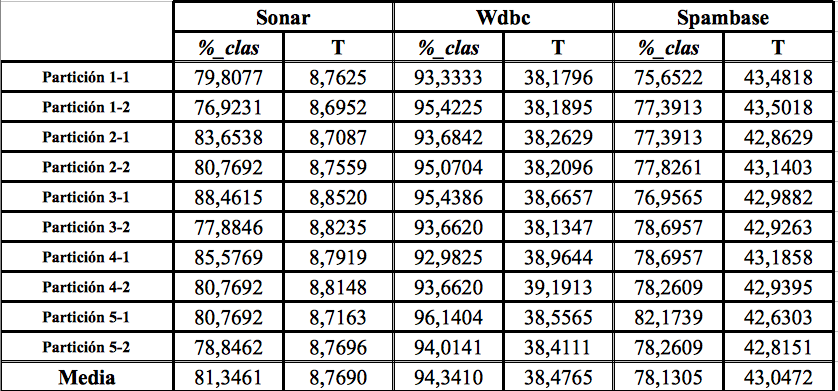
\includegraphics[scale=0.55]{AGG-CA.png}  
	
\end{figure}

\begin{figure}[H]
	\centering
	\caption{Resultados AGE-BLX} \label{fig: Resultados AGE-BLX}
	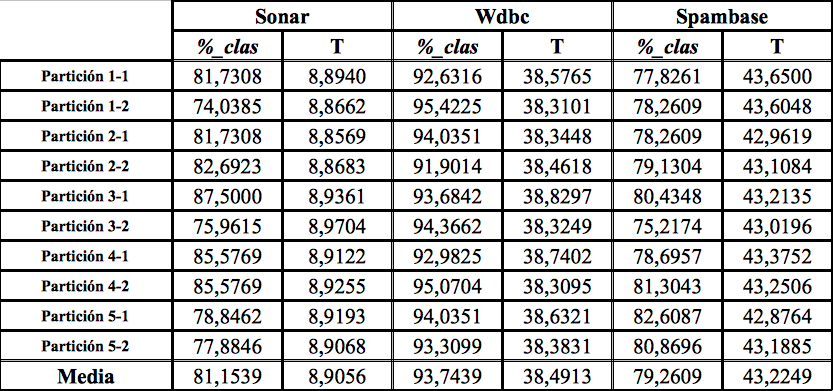
\includegraphics[scale=0.55]{AGE-BLX.png}  
	
\end{figure}

\begin{figure}[H]
	\centering
	\caption{Resultados AGE-CA} \label{fig: Resultados AGE-CA}
	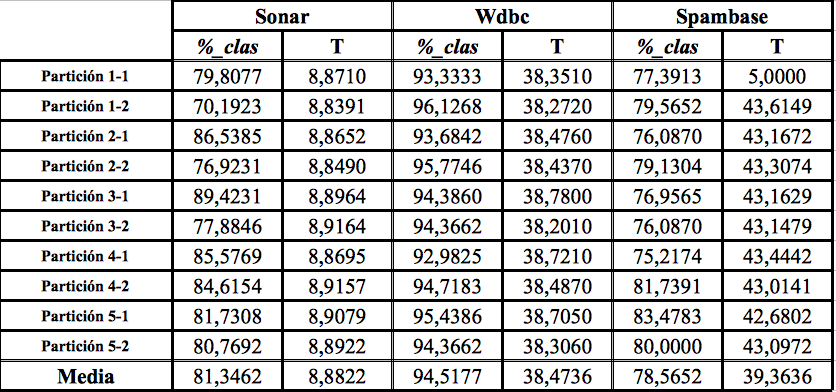
\includegraphics[scale=0.55]{AGE-CA.png}  
	
\end{figure}

\begin{figure}[H]
	\centering
	\caption{Resultados AM-1} \label{fig: Resultados AM-1}
	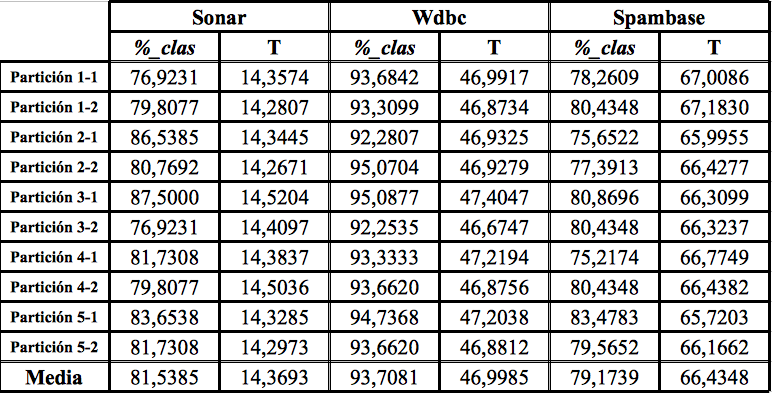
\includegraphics[scale=0.55]{AM-1.png}  
	
\end{figure}

\begin{figure}[H]
	\centering
	\caption{Resultados AM-01} \label{fig: Resultados AM-01}
	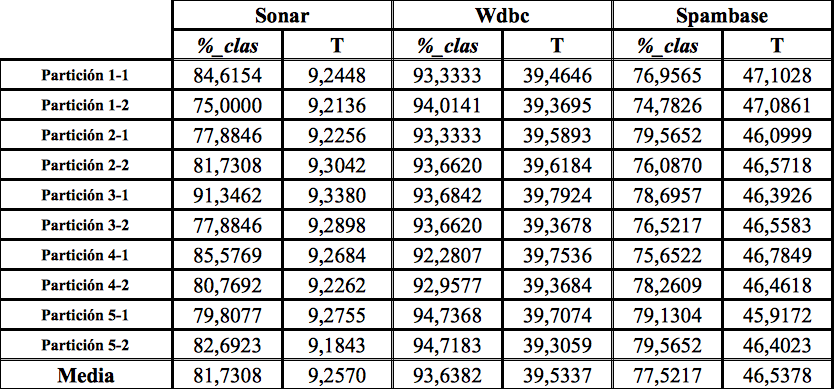
\includegraphics[scale=0.55]{AM-01.png}  
	
\end{figure}

\begin{figure}[H]
	\centering
	\caption{Resultados AM-01MEJ} \label{fig: Resultados AM-01MEJ}
	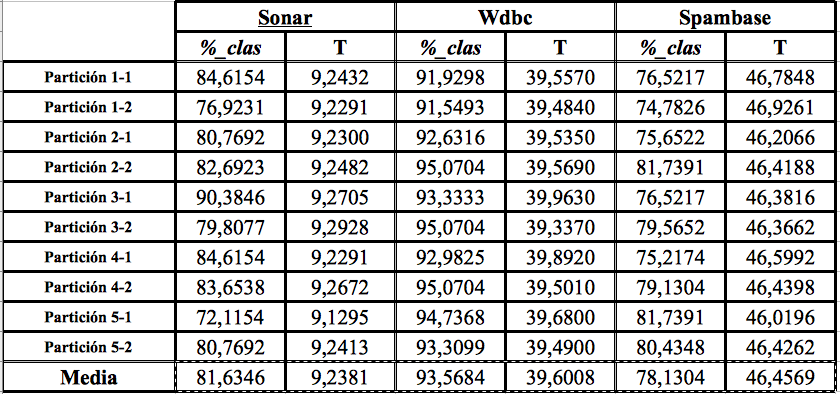
\includegraphics[scale=0.55]{AM-01MEJ.png}  
	
\end{figure}


Ahora pasemos a realizar una tabla comparativa con las medias, tanto de tiempo como de tasas obtenidas para cada uno de los algoritmos para poder realizar así un análisis de forma global:

\begin{figure}[H]
	\centering
	\caption{Comparativa global} \label{fig: Comparativa Global}
	\includegraphics[scale=0.55]{GLOBAL.png}  
	
\end{figure}

Realicemos ahora un anánisis de los datos obtenidos e intentemos razonar el porqué de dichos datos.\\ 

Si analizamos a primera vista las tasas obtenidas según los tres distintos conjuntos, lo primero que nos damos cuenta es de la gran importancia que tiene el mero hecho de que el conjunto de datos que usamos sea o no represntativo.\\ 
Por ejemplo, nos damos cuenta de que el conjunto de datos de cancer (Wdbc) es el que posee los datos más representativos de los tres, lo cuál facilita el aprendizaje. Es por eso que es en este en el que se obtienen las mayores tasas de clasificación, seguidas por las de Sonar y por último las de Spam. 
\subsection{Análisis genéticos}
Si nos centramos concretamente en la familia de algoritmos genéticos podemos observar, evidentemente, la necesidad elevada de cálculo en comparación con métodos Greedy como RELIEF, lo cual influye significativamente en el tiempo del algoritmo.\\ 
Por otra parte, los genéticos nos ofrecen la posibilidad de realizar exploración en el espacio de búsqueda, pudiendo de esta forma evitar máximos locales, como puede pasar con el RELIEF.\\ 

Es interesante observar con más profundidad los resultados obtenidos de algoritmos genéticos según
su esquema de evolución:

\subsection{Generacionales VS Estacionarios}
Si comparamos generacionales y estacionarios estrictamente observando la tabla, podríamos pensar que ambos son iguales, puesto que tanto los tiempos como las tasas obtenidas en los tres conjuntos no difieren apenas en unas décimas o incluso centésimas entre ellos.\\ 

Pero si analizamos la funcionalidad de ambos, podemos deducir que la principal diferencia entre estacionarios y generacionales es la diversidad que producen. \\ 
En esquema estacional, únicamente se reemplazan dos individuos como máximo en una nueva generación, e incluso puede pasar que no se reemplace ninguno (puesto que los hijos son peores que los peores individuos de la población actual) y obtengamos una generación igual a la anterior. \\ 

En cambio en el modelo generacional, el porcentaje de la población reemplazada por los descendientes es mucho mayor, en nuestro caso un 0.7 como hemos visto. Esto puede generar mayor diversidad a la hora de la generación de descendientes, ampliando así el espacio de búsqueda. \\ 
En cualquier caso, dependerá del tipo de problema que deseemos tratar, para así poder adecuar mejor un esquema de evolución u otro.

\subsection{BLX VS CA}
En una vista apriori sin comparar datos de los dos operadores de cruce, podríamos pensar que el operador BLX es mejor que el Cruce Aritmético por el hecho de ser más complejo y diversificar, en parte, con cierta componente aleatoria la reproducción de los padres.\\ 

Pero en la práctica, a la hora de la verdad, podemos ver que las tasas obtenidas por ambos son similares, incluso dependiendo del conjunto de datos aquellos con operador de cruce aritmético obtienen ligeramente mejores tasas, lo cuál nos lleva a hacernos la siguiente pregunta: ¿Complejidad implica mejora?, en este caso la más simple nos da casi las misma soluciones, pero con tiempos ligeramente menores, lo que implica que a veces lo sencillo es lo mejor, siguiendo el principio de la navaja de Ockham.

\subsection{Exploración VS explotación}

Si comparamos los resultados obtenidos por nuestro algoritmo de explotación (BL) con nuestros algoritmos genéticos, vemos que las tasas obtenidas por los genéticos son una o dos décimas superiores a las obtenidas por la búsqueda local. La principal razón de esto son los máximos locales.\\ 
El principal problema de la búsqueda local son los máximos locales, puesto que se trata de un algoritmo de explotación, es factible que se de el caso de que estemos explotando una determinada zona, obteniendo buenos resultados, pero estemos atascados en una cota local, de forma que no podamos llegar nunca a soluciones que se encuentran en distintas regiones del espacio de búsqueda.\\ 

Esto mismo tratan de solucionar los algoritmos de exploración. Se trata básicamente de sacrificar la obtención de una buena solución en una única región concreta del espacio de búsqueda, por una exploración más amplia del mismo.\\ 

Entonces, ¿que es mejor, sacrificar precisión por amplitud de miras, o lo contrario?.

Una buena solución es una hibridación entre explotación y exploración. Los algoritmos meméticos implementados nos permiten justo eso, realizar una exploración primero mediante un algoritmo genético, permitiendo así dirigirse a una región del espacio de búsqueda con buenas soluciones, y una vez allí aplicar una búsqueda local para realizar una exploración de este. De hecho, las tasas obtenidas por los meméticos son superiores a las obtenidas por una simple búsqueda local individual.

\section{Conclusión}
Como hemos visto en el análisis, la elección de un buen algoritmo de búsqueda es importantísima a la hora de la resolución de un problema, y se encuentra muy ligada a el ámbito de el mismo.\\ 

No existe un claro vencedor, puesto que como hemos dicho entran muchas variables en juego, dependientes en gran parte del dominio del problema.


%----------------------------------------------------------------------------------------
%	CODIGO EJEMPLO
%----------------------------------------------------------------------------------------

\begin{comment}


\begin{lstlisting}[language=bash, style=r]
warehouses=4
loadWorkers=4
terminals=1
//To run specified transactions per terminal- runMins must equal zero
runTxnsPerTerminal=0
//To run for specified minutes- runTxnsPerTerminal must equal zero
runMins=10
//Number of total transactions per minute
limitTxnsPerMin=300

//Set to true to run in 4.x compatible mode. Set to false to use the
//entire configured database evenly.
terminalWarehouseFixed=true
\end{lstlisting}

\end{comment}


%----------------------------------------------------------------------------------------
%	FIGURA
%----------------------------------------------------------------------------------------

\begin{comment}


\begin{figure}[H]
	\centering
	\includegraphics[scale=0.35]{cpu_utilization1.png}  
	\caption{Uso de la CPU, mejorado} 
\end{figure}


\end{comment}
%----------------------------------------------------------------------------------------
%	TABLA (ancho fijo)
%----------------------------------------------------------------------------------------

\begin{comment}

\begin{table}[htb]
\centering
\begin{tabular}{| p{2.2cm}| p{2.2cm} |  p{2.2cm} |}
\hline
\multicolumn{3}{|c|}{Europa} \\
\hline
\multicolumn{2}{|c|}{Localización} & Estado \\
\hline \hline
España & Madrid & Canada \\ \hline
España & Sevilla & EE.UU \\ \hline
Francia & París & Inglaterra \\ \hline
\end{tabular}
\caption{Tabla de ancho fijo.}
\label{tabla:Título de tabla}
\end{table}

\end{comment}


\bibliographystyle{plain} % hay varias formas de citar



\end{document}
